\chapter{System Design}

\section{Overview}
In this section, we will illustrate the entire system in detail. We will go through all the various technologies that were finalized from the technical review, where they are located in the project structure and what role they have in creating a fluid and realistic experience for the user. In Figure~\ref{image:SystemArch} we can see the high-level design of the project. Each component has a major role to play in creating this fluid experience and we will discuss how they were implemented in detail.

\begin{figure}[h!]
	\caption{System Architecture.}
	\label{image:SystemArch}
	\centering
	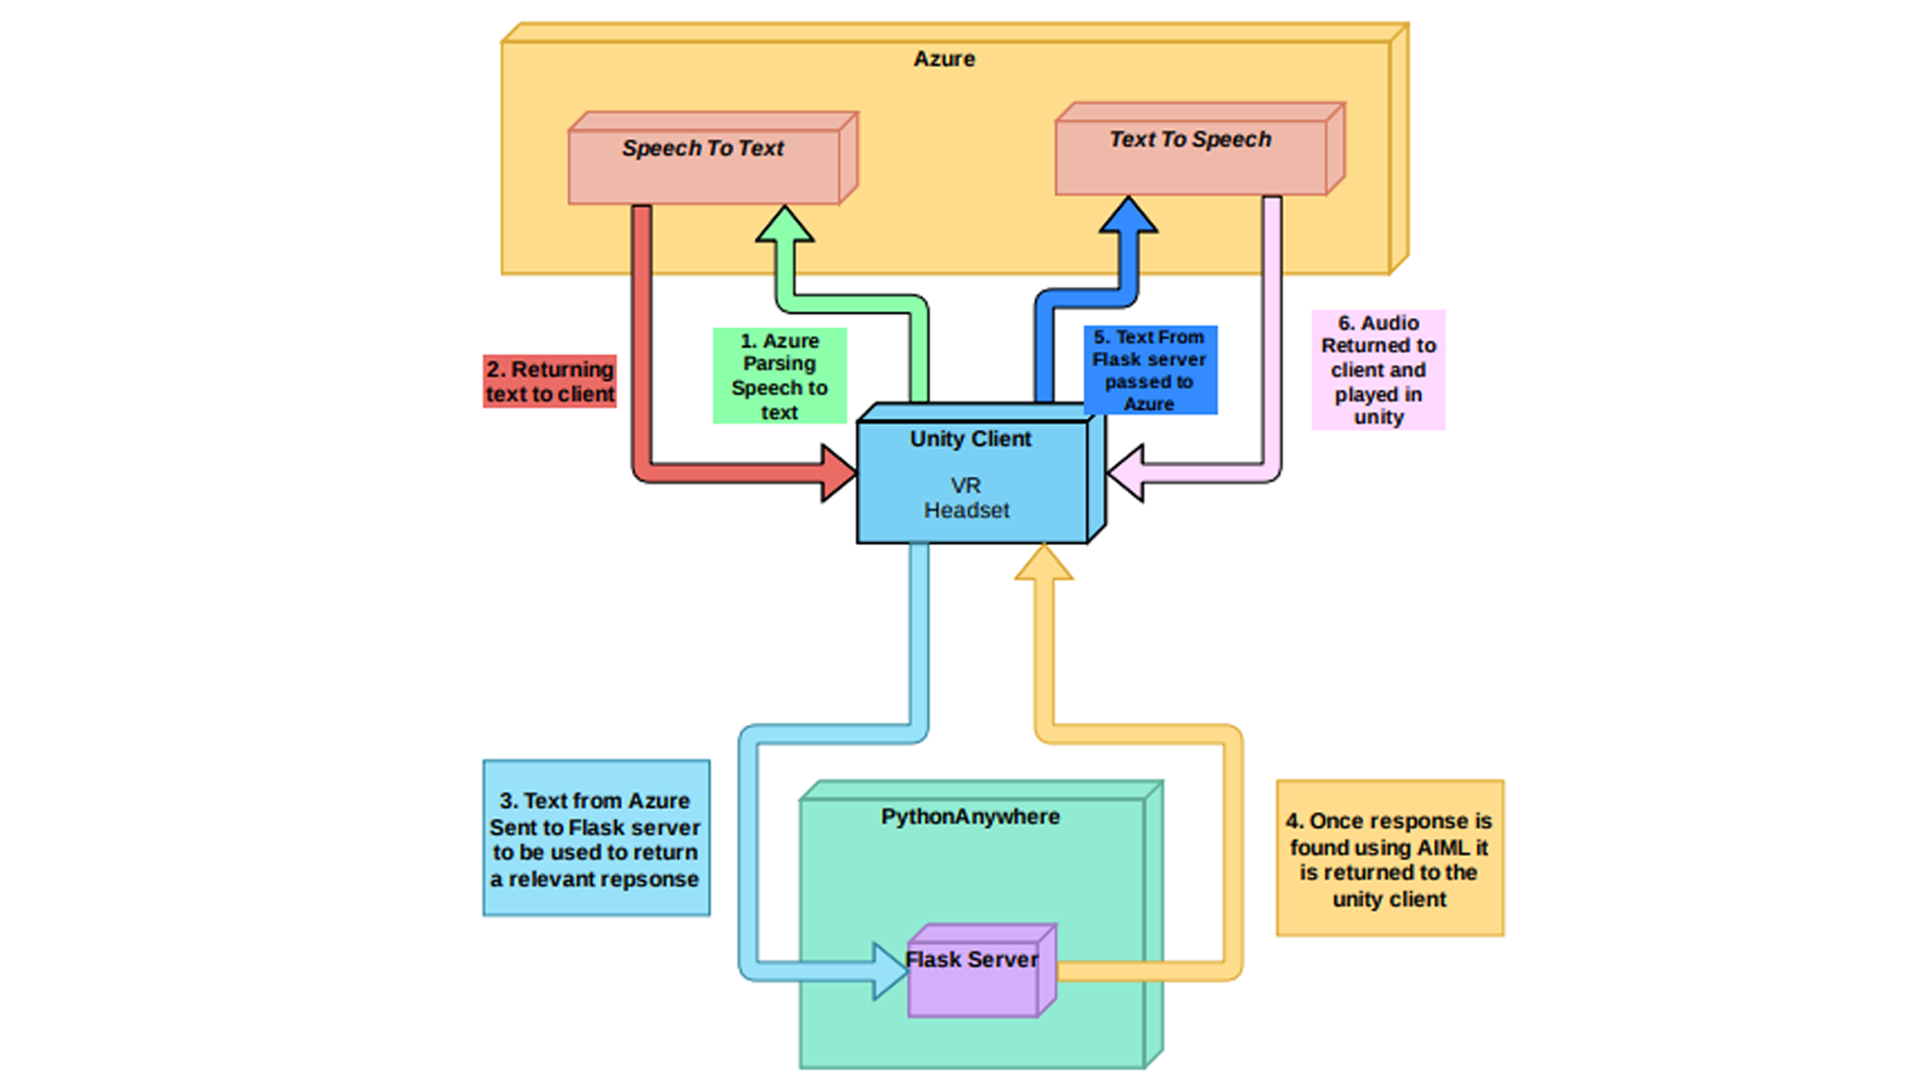
\includegraphics[width=1\textwidth]{Images/uml2.png}
\end{figure}

\section{Unity}
As seen in Figure~\ref{image:SystemArch} Unity is the central component in this application. It is the part that the user interacts with and the part where all the data flows in and out of. Having said that, in this section we will discuss the more graphical side of the implementation and how we did that.

\begin{figure}[h!]
	\caption{Unity Project Class Diagram.}
	\label{image:ClassDiagram}
	\centering
	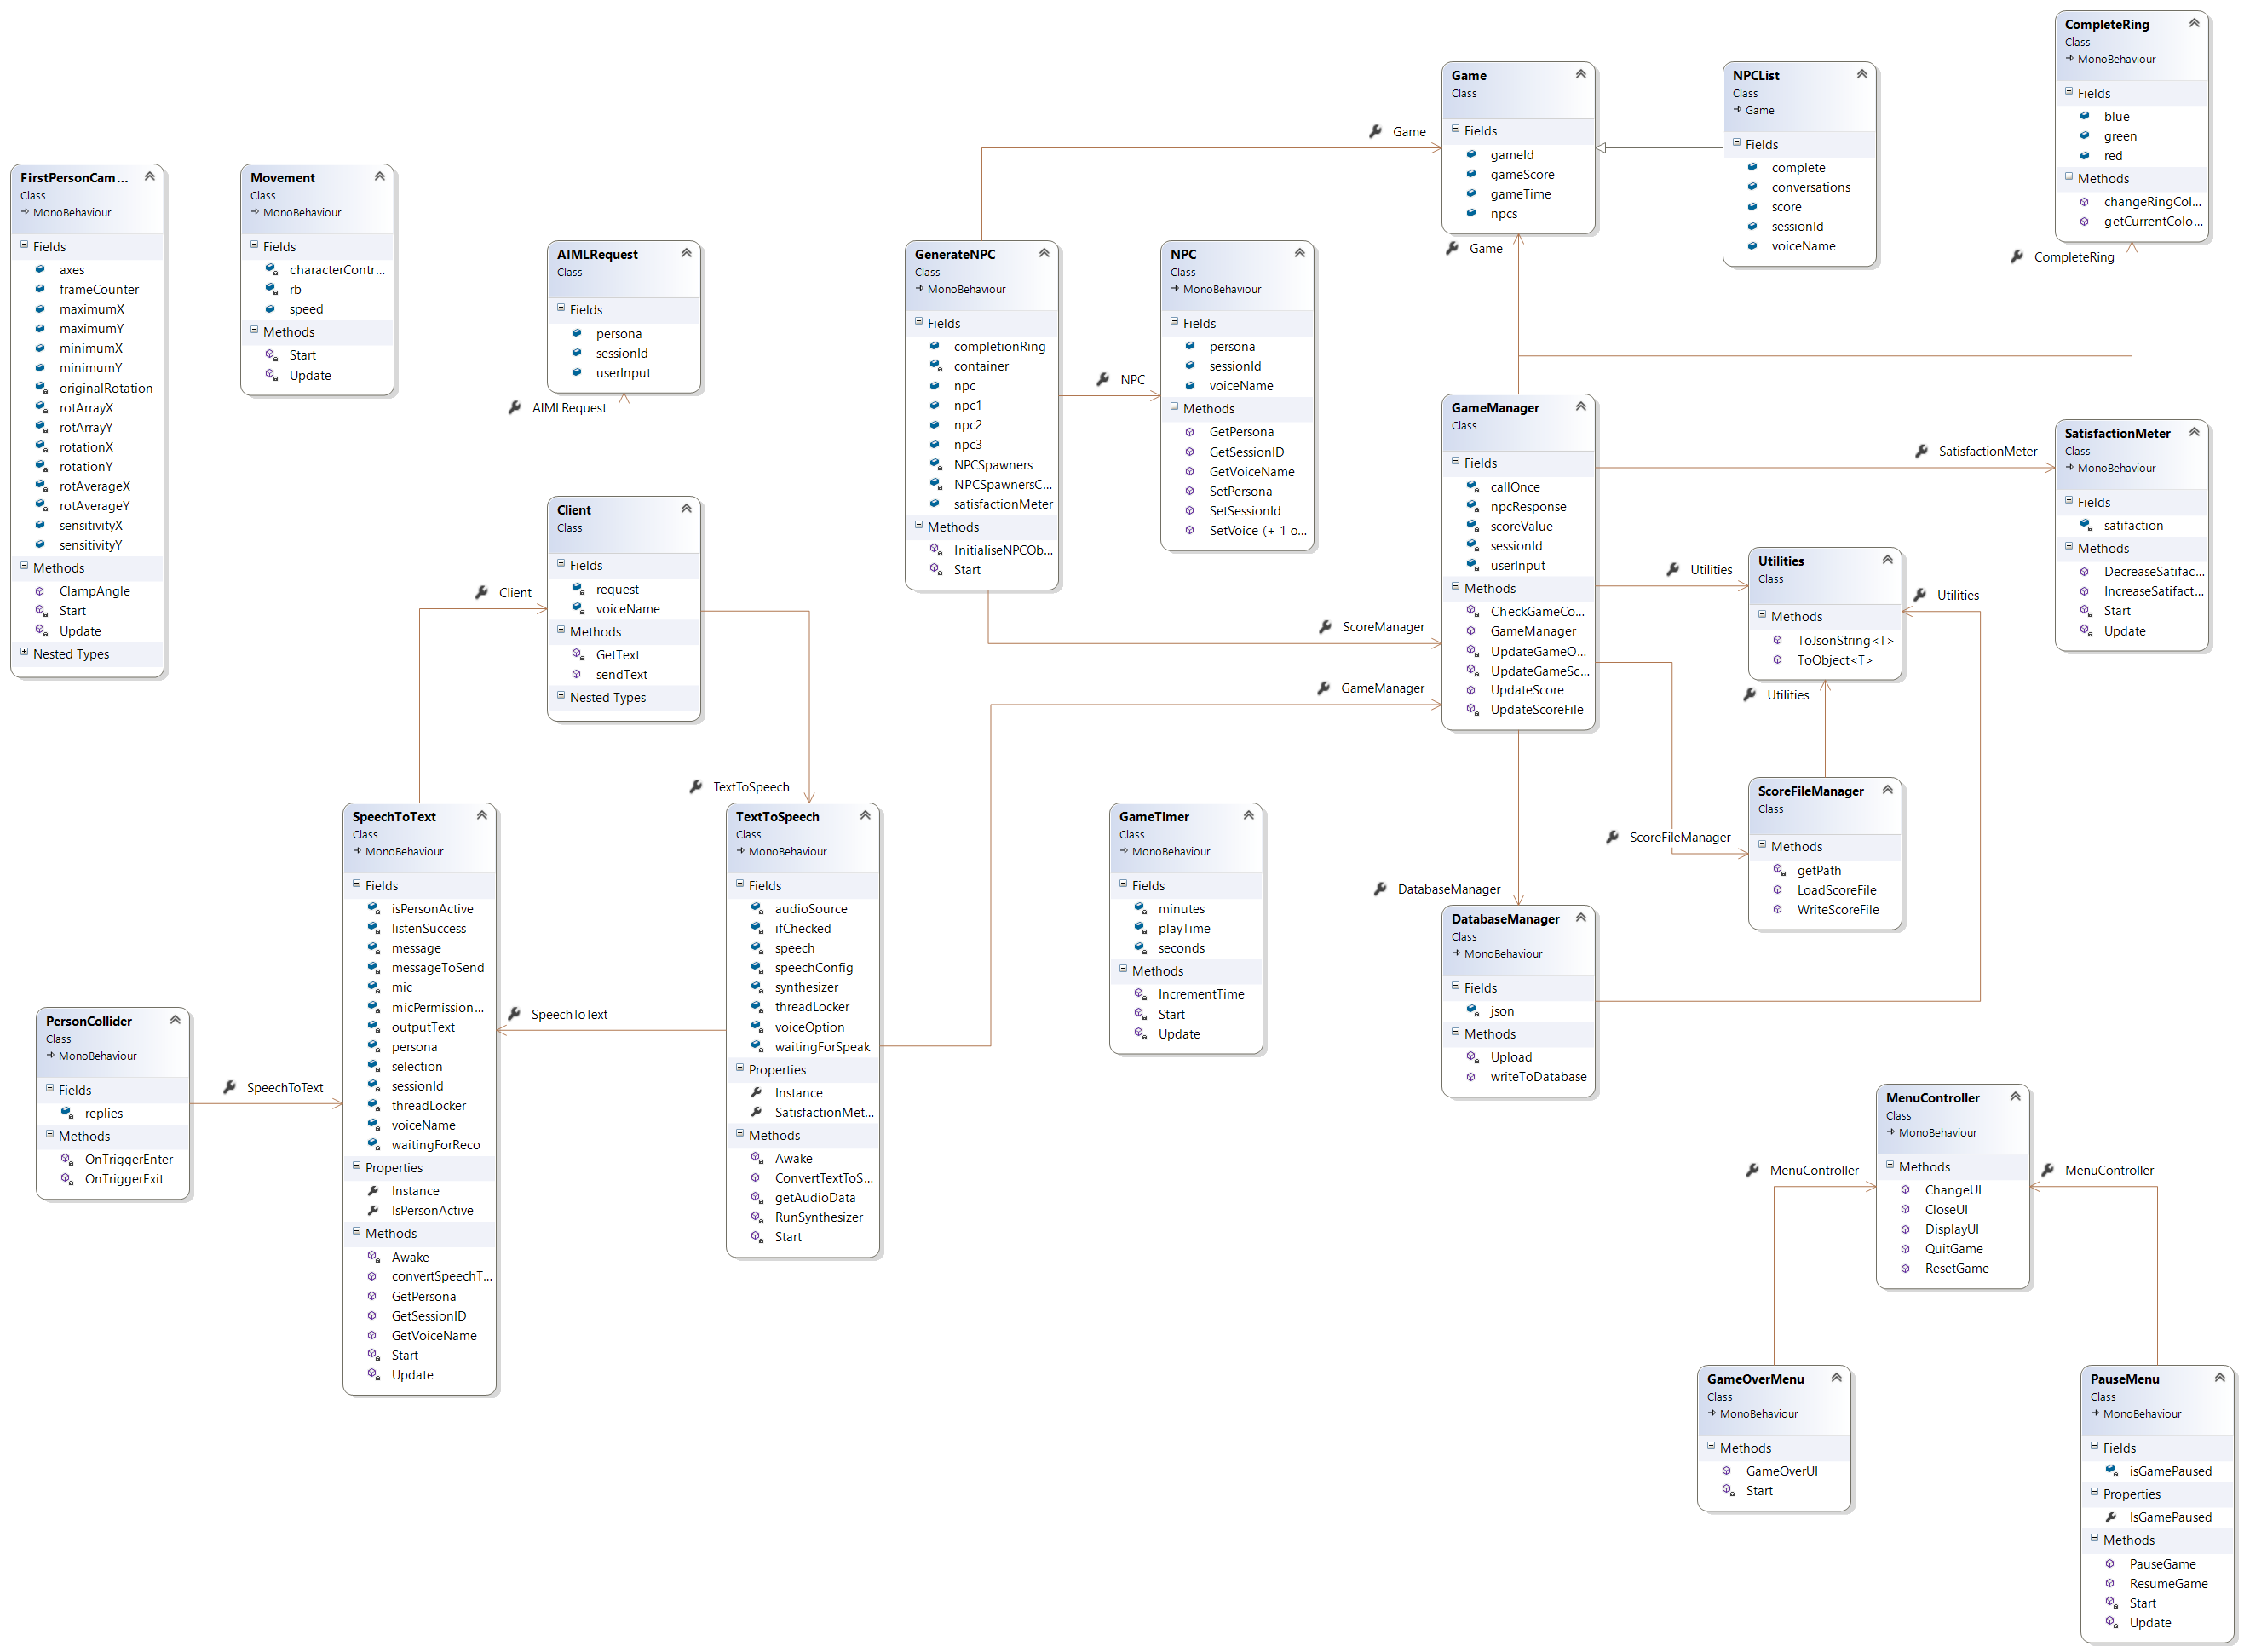
\includegraphics[width=1\textwidth]{Images/ClassDiagram.png}
\end{figure}

\subsection{3D Models}
Generating realistic bots with realistic models was a problem that was easily solved with the aid of a website called "http://mixamo.com/". This website has an plethora of high quality 3d character models along with animations. Once the model was imported into Unity all that was left to do was give these bots a session ID, random voice, gender based on that voice and a random persona E.g. Polite, neutral and rude. These personas would aid us later in deciding which AIML file to use server-side. As seen in the below code snippet this is how we generate all these traits. The session ID is a random number between 1 and 10000. The persona is an integer between zero and three, each number meaning a different persona: 

\begin{table}[!ht]
    \centering
\begin{tabular}{ |p{3cm}|p{5cm}|  }
\hline
\multicolumn{2}{|c|}{NPC Personas} \\
\hline
Number & Persona \\
\hline
0 & Rude NPC \\
\hline
1 & Neutral NPC \\
\hline
2 & Polite NPC \\
\hline

\end{tabular}
    \caption{Personas}
    \label{tab:my_label}
\end{table}


\begin{lstlisting}[language=python]
    
    public void SetSessionId()
    {
        sessionId = UnityEngine.Random.Range(1, 10000);
    }
    public void SetPersona()
    {
        persona = UnityEngine.Random.Range(0, 3);
    }
    public void SetVoice()
    {
        //0 = male 1= female
        int gender = UnityEngine.Random.Range(0, 2);
        Debug.Log("GENDER:" + gender);
        string[] voicesMale = {"en-US-GuyNeural", "en-IE-Sean"};
        string[] voicesFemale = { "en-US-JessaNeural", "de-DE-KatjaNeural" };
        if (gender == 0)
        {
            int rand = UnityEngine.Random.Range(0, voicesMale.Length);
            voiceName = voicesMale[rand];
        }
        else if(gender == 1)
        {
            int rand = UnityEngine.Random.Range(0, voicesFemale.Length);
            voiceName = voicesFemale[rand];
        }
    }
\end{lstlisting}

Once these traits have been generated all that is left to be done is to generate them in the virtual 3D environment. The solution to this can be seen in the below snippet.
This snippet is also wrapped in a for loop to generate multiple random NPCs. There is an array of manually place GameObjects in the virtual world. These GameObjects act as spawning points for a single NPC. Based on the NPCs voice a Male or Female model is loaded then it is spawned in the position and rotation of one of the spawn points according to the index of the loop. After this process is complete, we see NPCs standing in all the spawn points. This is how all the NPCs/Bots are spawned in the application.\newline

\begin{lstlisting}[language=python]
    if (copy.GetComponent<NPC>().GetVoiceName() == "en-US-JessaNeural" || copy.GetComponent<NPC>().GetVoiceName() == "de-DE-KatjaNeural")
    {
        int rand = UnityEngine.Random.Range(0, 2);

        if(rand == 0)
        {
            copy = Instantiate(npc2, new Vector3(NPCSpawners[i].position.x, NPCSpawners[i].position.y, NPCSpawners[i].position.z), Quaternion.Euler(0, NPCSpawners[i].rotation.eulerAngles.y, 0));
            copy.GetComponent<NPC>().SetVoice(npcVoice);
            copy.transform.parent = container.transform;
        }else if(rand == 1)
        {
            copy = Instantiate(npc3, new Vector3(NPCSpawners[i].position.x, NPCSpawners[i].position.y, NPCSpawners[i].position.z), Quaternion.Euler(0, NPCSpawners[i].rotation.eulerAngles.y, 0));
            copy.GetComponent<NPC>().SetVoice(npcVoice);
            copy.transform.parent = container.transform;
        }
    }
    else
    {
        copy = Instantiate(npc1, new Vector3(NPCSpawners[i].position.x, NPCSpawners[i].position.y, NPCSpawners[i].position.z), Quaternion.Euler(0, NPCSpawners[i].rotation.eulerAngles.y, 0));
        copy.GetComponent<NPC>().SetVoice(npcVoice);
        copy.transform.parent = container.transform;
    }
\end{lstlisting}

\subsection{Animation}
Animations in our opinion were important in this application. We needed the user to feel as if they were speaking to a person. If the NPCs where static it would have ruined the realism, completely disconnecting the user from this virtual world. As mentioned earlier, we were fortunate to find a website called Mixamo. As well as realistic models it also had animations to go alongside them. The process of applying the animation to the model is simple but tedious. Firstly, you must add an Animator component to the model/NPC this allows you to manage your animation clips. Once this is done, animations can be added to the animator using a graph-like interface as seen in Figure~\ref{fig:anim}. Each animation is considered as a state. If certain parameters are met you can change the state, therefore changing the animation.

\begin{figure}[!ht]
    \centering
    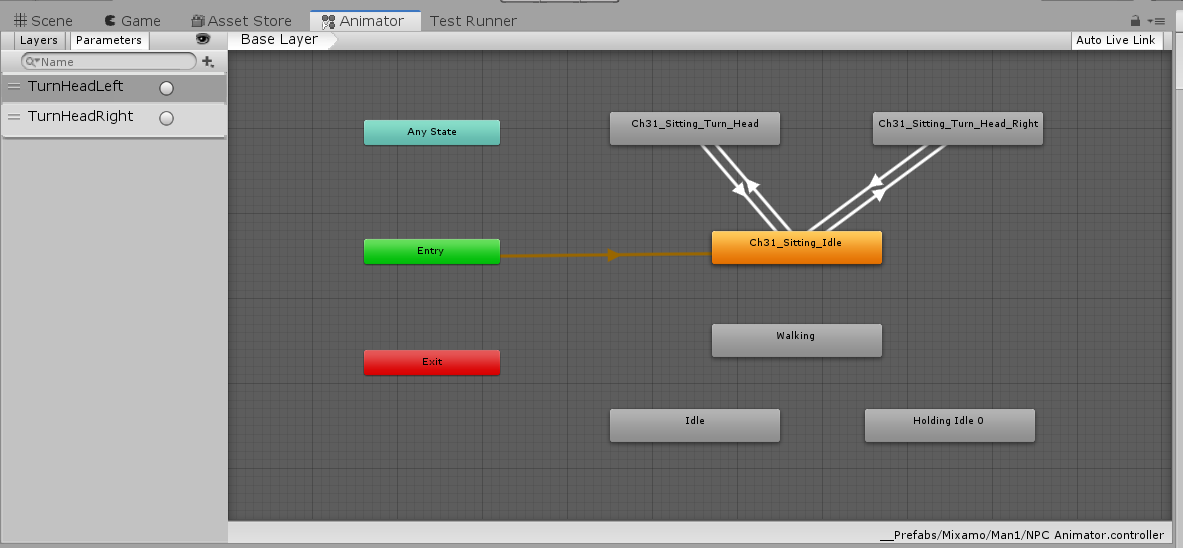
\includegraphics[width=1\textwidth]{Images/animator.PNG}
    \caption{Animator}
    \label{fig:anim}
\end{figure}

\subsection{Usability/User Experience}
Throughout the development of this project we focused a lot of effort on ensuring the training application was intuitive to the user. We looked a number of areas in regards to user experience and usability which we will look at below.

\subsubsection{Passenger (NPC) Interaction}
From our initial meetings with our supervisor and the initial scope we laid out we felt getting the interaction to feel as real and immersive as possible was important. In real life a ticket inspector can walk up to passenger and start a conversation simply by saying "Hello". We wanted our training experience to reflect this simple nature. There were a number of interaction in our development process such as initially having the player press a button to start speaking with an NPC, but we felt it wasn't quite cumbersome and took away from the experience especially in VR. Through user testing we developed a simple way of interacting with an NPC. It involved adding a collider to each NPC which would act as a barrier. Once this barrier was passed, E.g the player moves close to the NPC it would trigger a conversation and the Azure Speech to Text service would start listening for input. Another aspect we looked at was keeping the flow of conversation intuitive. Similar to the initial interaction we felt that pressing a button wasn't suitable, so again we developed an automatic system. Once the result is returned from the Text to Speech and spoken by the passenger, the STT service will automatically start listening again for the player reply to the passenger. For example if the player asked to see the passengers ticket, and the NPC replied with "I don't have a ticket", then the service will start listing for possible reply like "Why don't you have a ticket?". This simple flow of interaction and conversations improved the user experience drastically. More information on STT and TTS technologies can be found below in their respective sections. 

\subsubsection{Player Input}
Again from our meetings another area to improve immersion was to all the player to psychically speak to a passenger. Our initial tests involved a keyboard input however it was very slow and cumbersome to type out each reply. We also looked at a multiple choice decisions where the player could reply with three options, however from initial user tests it was compared to a role playing decision based game rather than a immersive training experience. Instead we developed a Speech service that would listen for your voice, parse it to text to send to our chatbot for a reply. Of course this was more of a challenge as the player could say anything and in any way, however it is something that was very successful in our final build and really improved the overall experience.

\subsubsection{Passenger Information and Scoring}
There were a number of things that we wanted to display to the player about each passenger they interact with. Firstly, whether the passengers ticket had been checked on not. We decided this should be simple and researched multiple methods such as displaying a green tick beside their head and outputting a completion sound to the user amongst others. We decided that a ring around the passengers feet that would initially be red and then turn to green would work best. The ring turns to green when the player has checked the passengers ticket or dealt with situation where they don't have a ticket. It also turns blue when the player is within the range to start a conversation. This simple red, blue green loop is very simple to grasp and worked well in the various user tests. Also it worked well for the VR experience as it is very subtle but effective in displaying the required information.

\subsubsection{VR Support}
As our main platform focus was VR support on the Oculus Quest we wanted to ensure it was the most immersive experience possible. This was taken into account when designing the various environments (The train, the station, city etc), the in game sound, the player interactions, and controls. The controls were designed to require the least requirement of buttons possible, so the user didn't feel like they were holding controllers. All menu interactions are done by looking around in the virtual space and pulling the triggers, which is a simple fluid movement. One area we felt really improves the experience was the inclusion of the in-game watch. It was a very simple thing but it really was success in our user tests. In the virtual space we wanted to feel like the user is really in the train station to the best possibility, and if they look down at anytime they can view their hands in real time and move their fingers. On the left hand there is a simple dial watch that displays the real world time. If the user touches this watch with their right hand the game is paused and a virtual menu is displayed. Unfortunately, this was only a feature that could work on the VR build, but we implemented the pause menu support by displaying the menu on front of the player when the pause button is pressed.

\subsubsection{User Interface (UI) Design}
For this project we used a simple design scheme for all menus and UI. It involved a simple grey background, strong contrasting text and blue buttons. This made it easy to read and view all elements throughout the application. All menus were also designed with ergonomics in mind, so that it would be easy for the user to move between menus, close the menus or select options. For example on the pause menu implemented in VR the QUIT and RESET button were placed at the top as from testing they could be accidentally pressed when touching the watch. The score and game time is also placed accordingly along with the option to turn he sound on and off. We wanted to insure everything required by the player is all in one place and easily accessible. This idea was reflected in the start menu and game over menu too.

\subsubsection{Tutorial}

% Interactions with npcs and placement
% Speech rather than keyboard input
% Menus / Layout
% If ticket is checked
% VR controls
% Pause menu on watch

% Tutorial

\begin{figure}[h!]
	\caption{Menus Class Diagram.}
	\label{image:Menus}
	\centering
	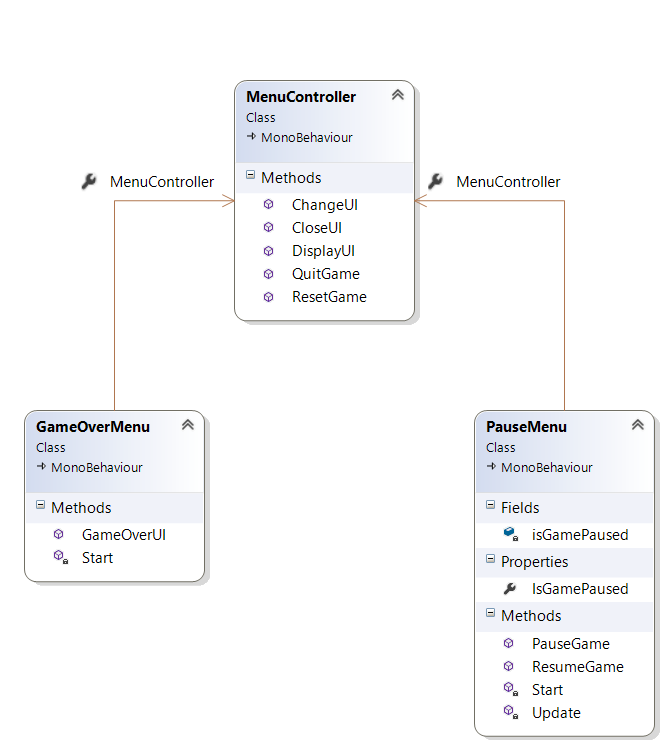
\includegraphics[width=0.8\textwidth]{Images/ClassDiagram Menus.png}
\end{figure}

\subsection{Scoring System}
As one of the main goals of this project was to create a useful training experience to train ticket inspectors in relation to conflict resolution, we decided it would need a scoring system to help both the trainee and the training centre. A simple system was devised for each interaction and was scored depending on user input and the way it's said. Table ~\ref{tab:scores} shows example of how the result is scored, based on the user input. If the user is deemed aggressive then they will get a -1 score, if they are deemed neutral their score won't change and if they are deemed positive they will gain one point to their total score. This simple system proved beneficial in early tests, so we implemented same idea with the personalities of each NPC.

\begin{table}[!ht]
    \centering
\begin{tabular}{ |p{6cm}|p{2cm}|  }
\hline
\multicolumn{2}{|c|}{Interaction Scoring} \\
\hline
User Input & Score \\
\hline
Show me your ticket! & -1 \\
\hline
Can I see your ticket? & 0 \\
\hline
Can I see your ticket, please? & +1 \\
\hline

\end{tabular}
    \caption{Scores}
    \label{tab:scores}
\end{table}

The scoring systems works as follows as seen in Figure~\ref{image:Scoring}. Once the game is started and each NPC is being generated and template "Game" object is setup, this object contains a nested list "NPCList" which contains information about each NPC such as the conversations, current score, and sessionID. Once created it is written to a local file on the device, the decision to use file storage rather than have the object in memory was chosen for several reasons. Firstly, it allowed the file to be accessed at any time from any class easily, quickly and efficiently. It also would be stored if the game crashed, or if the user quit however results retrieval weren't implemented in the final build, however it would be something to look at for future development.

\par
\medskip

The next steps occur after each successful interaction with a NPC. The GameManager is called from the Client to update the game and score. The UpdateScore() method updates the score by reading in the current file, finding the NPC and updating their current score respectively. This also handles the check if the NPC is complete E.g. if their ticket has been checked. If the NPC is on the last state a boolean "complete" will be set to true which is used to check if the training experience is complete. This is written back out to a local file as a JSON string using the Utilities class methods. The Utilities methods were designed using generics so they can handle any type for usability. The end game condition is also checked here to see if the game is complete, if so, the end game menu is displayed with the players results.

\begin{figure}[h!]
	\caption{Scoring System Class Diagram.}
	\label{image:Scoring}
	\centering
	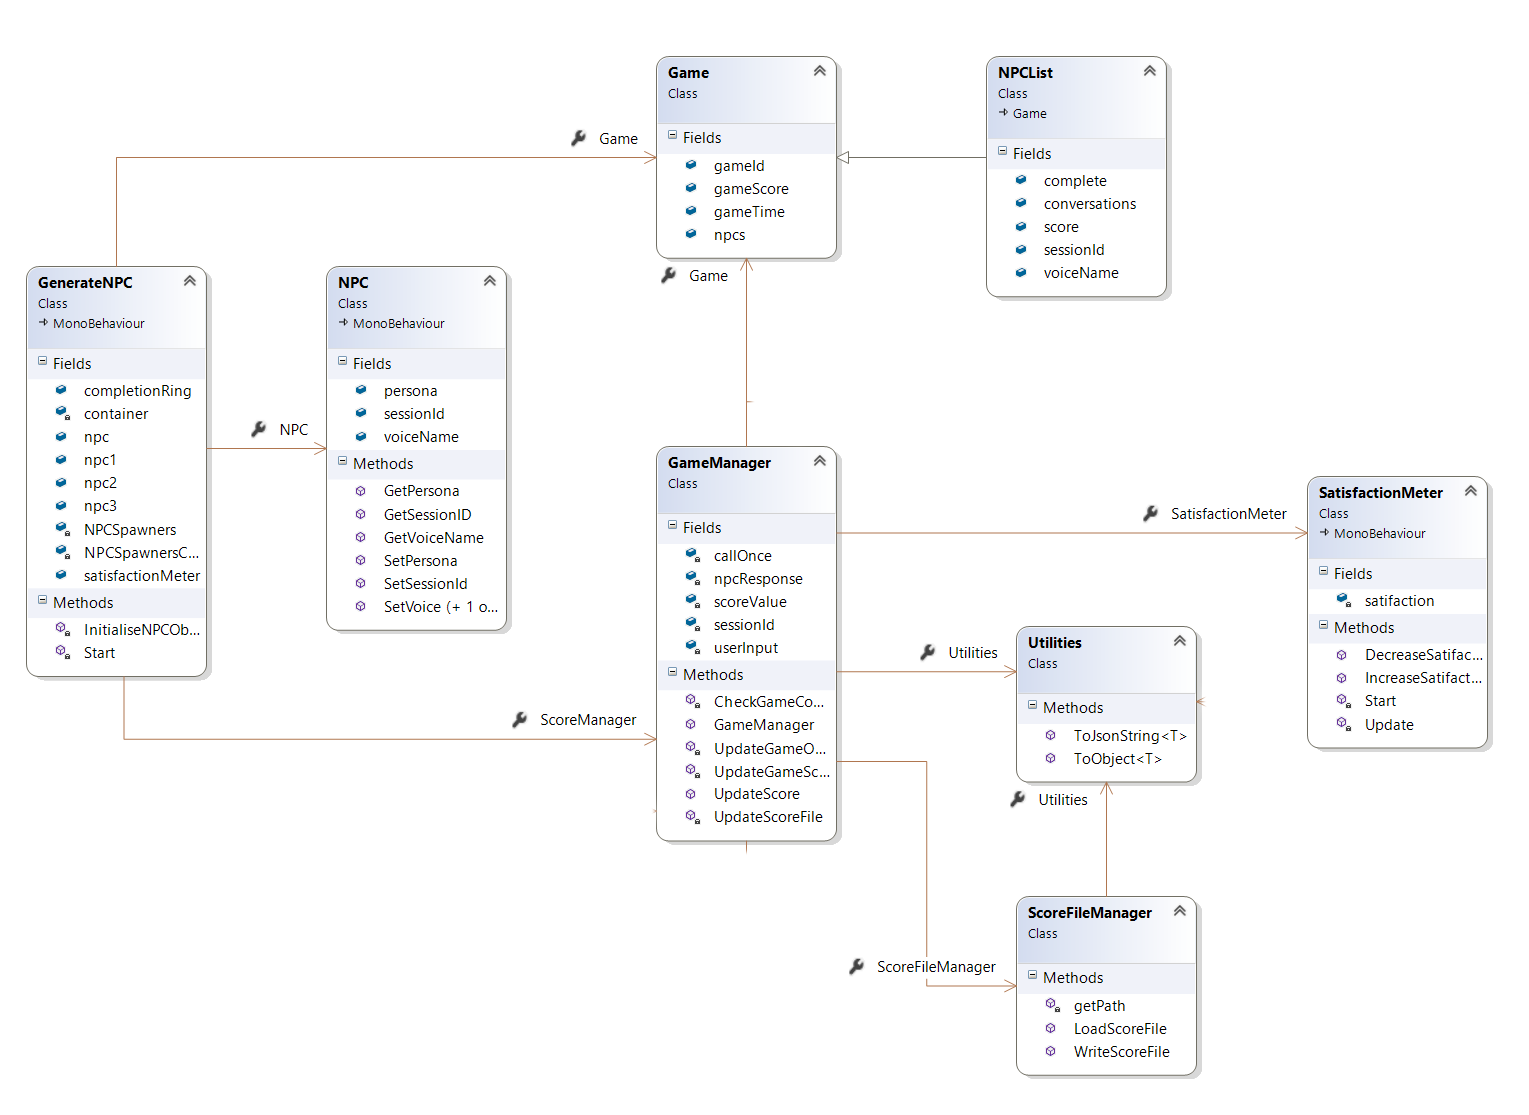
\includegraphics[width=1\textwidth]{Images/ClassDiagram Scoring.png}
\end{figure}

\subsection{Other Game Functions}

\section{Azure Speech Services}
From our research and testing efforts as laid out in the technology review Azure was chosen as the provider for the speech services due to its many benefits. This provided the voice of our human like NPC's (Non-player character) and converted the players speech to machine readable diction which is sent to the Flask server for processing. Azure provides a Unity plugin to allow access to their services, with this implemented we could access the classes required.

\par
\medskip

The Speech to Text and Text to Speech functionality were the first sections to get working as it was initially decided that we would use voice commands and human speech to improve the user experience and usability rather than having the user type in their response. Using the sample Unity project provided by Microsoft as a guide we tested the implementation to learn how it works. Using this an initial prototype was built where the player could walk up to a cylinder which would turn blue on interaction. Once the collision occurs the speech engine begins listening and the result is returned from an Azure server as text output to the screen. We also developed a similar test build for Text to Speech where a user could input text into a text box which would play back their input as if it was spoken by a human voice. This was one of the bare essential goals of our project.

\par
\medskip

Figure~\ref{image:SpeechServices} shows the class diagram of the whole speech services in the project. The process starts in the PersonCollider class, once the player interacts with the NPC OnTriggeredEntered is fired, which sends a request to the SpeechToText class. This begins listening and displays this to the user. Once speech is recognised it is sent to Azure for processing and a result is returned as text. This is then sent to the Client which sends a HTTP request to the server as an AIMLRequest object. Once the result is processed the text is returned with a score for the chatbot to speak and the game will be updated. The TextToSpeech class handles this asynchronously and the process restarts again once the chatbot is finished talking (TTS). We will now go into more detail of how this three elements work.

\begin{figure}[h!]
	\caption{Speech Services Class Diagram.}
	\label{image:SpeechServices}
	\centering
	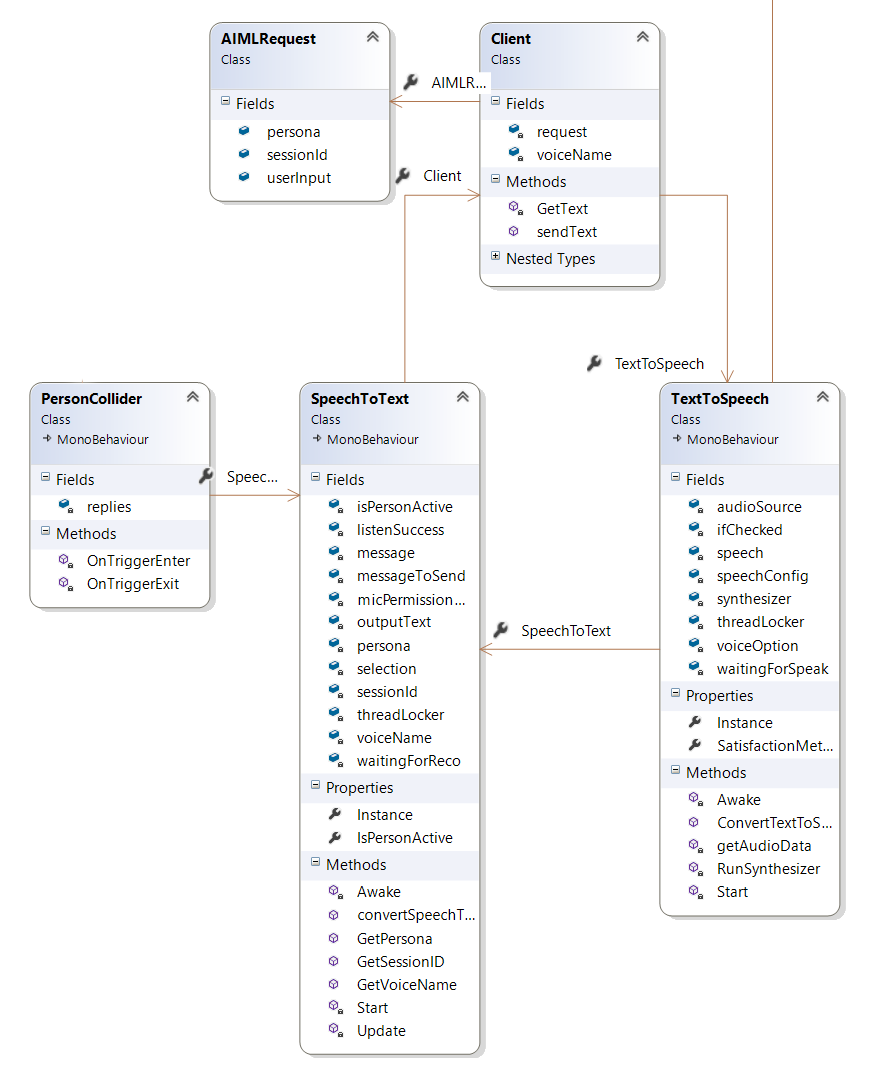
\includegraphics[width=0.8\textwidth]{Images/ClassDiagram STT and TTS.png}
\end{figure}

\subsection{Speech-to-Text}
Once this class is called a connection to the Azure services is made, then with a using statement to cut down memory usage the configuration information is passed into the imported classes (SpeechRecognizer). This begins listening for a total of 15 seconds in which it will timeout and display an error to the user. If the speech recognition is successful, the message is saved and will be sent to the client on the next update. This can be seen in Listing~\ref{lst:STT}.

\par
\medskip

Throughout the duration of the project the SpeechToText code was modified heavily to improve it in many ways, which is described below.

\begin{itemize}
  \item We had to implement a web client so it could contact the server via HTTP. More information can be found in the HTTP section in regard to the web client. We ran into problems trying to call the web client on result returned (Line 24 in Listing~\ref{lst:STT}) so instead a check was added to the Update method which checks if there is a message to be sent on each frame. If so then the returned result is sent to the server for processing.
  \item We also worked on making this Speech To Text class threaded so it would let the application continue to play when waiting for a result, as seen on line 10-13 in Listing~\ref{lst:STT}.
  \item Security was implemented by protecting the key from external access, so it is local to the device.
  \item Singleton design pattern was used as there should only be one instance of SpeechToText and it allows easy access from other classes.
\end{itemize}

\begin{lstlisting}[caption={Speech To Text - Setup and request},label={lst:STT},language=python]
// Creates an instance of a speech config with specified subscription key and service region.
// API_Key for security this is read in from a text file and is not included on Github. 
var config = SpeechConfig.FromSubscription(API_Key, "westeurope");

using (var recognizer = new SpeechRecognizer(config))
{
    listenSuccess = false;
    messageToSend = "";

    lock (threadLocker)
    {
        waitingForReco = true;
    }

    // Starts speech recognition and returns after a single utterance is recognized. The end of a
    // single utterance is determined by listening for silence at the end or until a maximum of 15
    // seconds of audio is processed.  The task returns the recognition text as result.
    var result = await recognizer.RecognizeOnceAsync().ConfigureAwait(false);

    // Checks result.
    string newMessage = string.Empty;
    if (result.Reason == ResultReason.RecognizedSpeech)
    {
        newMessage = result.Text;

        // Set independant variables for sending the message to the server.
        listenSuccess = true;
        messageToSend = newMessage;
    }
    else if (result.Reason == ResultReason.NoMatch)
    {
        newMessage = "NOMATCH: Speech could not be recognized.";
    }
    else if (result.Reason == ResultReason.Canceled)
    {
        var cancellation = CancellationDetails.FromResult(result);
        newMessage = $"CANCELED: Reason={cancellation.Reason} ErrorDetails={cancellation.ErrorDetails}";
    }

    lock (threadLocker)
    {
        message = newMessage;
        waitingForReco = false;

        // Dispose of recognizer correctly.
        recognizer.Dispose();
    }
}
\end{lstlisting}

\subsection{Text-to-Speech}
Once this class is called a connection to the Azure services is made using the configuration information. This includes data such as the voice name which is passed from the Client. There are several voices available both male and female for different countries in the world to give a more realistic and unique experience. We choose two male and female voices from the list of Neural voices which are created using machine learning, from testing they provided the most realistic sounding voice. This can be seen in Listing~\ref{lst:TTS1}. Once setup the text is passed into the synthesizer.SpeakTextAsync() function. This is implemented using a task (Task<SpeechSynthesisResult>) so it doesn't block and wait for a response.

\begin{lstlisting}[caption={Text to Speech - Setup and request},label={lst:TTS1},language=python]
public void ConvertTextToSpeech(string inputText, string voiceName, bool ifChecked)
{
    this.ifChecked = ifChecked;

    // For security this is read in from a text file and is not included on Github. 
    string API_Key = System.IO.File.ReadAllText("../../API_Key.txt");

    speechConfig = SpeechConfig.FromSubscription(API_Key, "westeurope");
    
    // The default format is Riff16Khz16BitMonoPcm.
    // We are playing the audio in memory as audio clip, which does not require riff header.
    // So we need to set the format to Raw16Khz16BitMonoPcm.
    speechConfig.SetSpeechSynthesisOutputFormat(SpeechSynthesisOutputFormat.Raw16Khz16BitMonoPcm);

    // Change voice depending on option selected for multiple characters of different genders and ethnicities.
    speechConfig.SpeechSynthesisVoiceName = voiceName;

    lock (threadLocker)
    {
        waitingForSpeak = true;
    }

    // Creates a speech synthesizer.
    synthesizer = new SpeechSynthesizer(speechConfig, null);

    // Starts speech synthesis and returns after a single utterance is synthesized.
    // There was an issue where the game would freeze at this point "synthesizer.SpeakTextAsync(inputText)" blocks until the task is complete. 
    // To solve this, I have implemented a task which runs using a Coroutine that waits until the result from Azure is returned. 
    // Code is adapted from: https://stackoverflow.com/questions/57897464/unity-freezes-for-2-seconds-while-microsoft-azure-text-to-speech-processes-input
    Task<SpeechSynthesisResult> task = synthesizer.SpeakTextAsync(inputText);

    StartCoroutine(RunSynthesizer(task, speechConfig, synthesizer));

    lock (threadLocker)
    {
        waitingForSpeak = false;
    }
}
\end{lstlisting}

\par
\medskip

The audio response received from Azure is 16-bit mono format. The 16 bit is the bit depth, or resolution of audio. A common compact disc (CD) uses 16 bits per sample. As it's returned as bits it must be converted first to a float array to be output to the device speaker. A loop was implemented to shift the bits left on each iteration using the formula supplied in the documentation. This can be seen on line 7 in Listing~\ref{lst:TTS2}. Once completed the audio is ready for output.

\begin{lstlisting}[caption={Text to Speech - Converting audio from bits to array},label={lst:TTS2},language=python]
private Task<float[]> getAudioData(SpeechSynthesisResult result)
    {
        var sampleCount = result.AudioData.Length / 2;
        var audioData = new float[sampleCount];

        for (var i = 0; i < sampleCount; ++i) {
            audioData[i] = (short)(result.AudioData[i * 2 + 1] << 8 | result.AudioData[i * 2]) / 32768.0F;
        }

        return Task.FromResult(audioData);
    }
}
\end{lstlisting}

The last step of the process is to output the processed audio directly to the device speaker. A clip is first created using the data and applied to the AudioSource of the NPC and then this is played as seen in Listing~\ref{lst:TTS3}. Lastly, the SpeechToText class is called again to start the NPC listening for a new user input. However, if the NPC's ticket has already been checked this step is skipped and a predefined output is spoken, E.g "Sorry, but you have already checked my ticket.".

\begin{lstlisting}[caption={Text to Speech - Asynchronous Audio Processing},label={lst:TTS3},language=python]
private IEnumerator RunSynthesizer(Task<SpeechSynthesisResult> task, SpeechConfig config, SpeechSynthesizer synthesizer)
{
    // Wait until the task is complete E.g Azure Text to Speech returns a result.
    yield return new WaitUntil(() => task.IsCompleted);

    var result = task.Result;
    
    // Check result.
    if (result.Reason == ResultReason.SynthesizingAudioCompleted)
    {
        // Create a task to create audio data and wait till its completed.
        Task<float[]> audioTask = getAudioData(result);
        yield return new WaitUntil(() => audioTask.IsCompleted);

        // Synthesize the Audio and play to the speaker.
        // The output audio format is 16K 16bit mono
        var sampleCount = result.AudioData.Length / 2;
        var audioClip = AudioClip.Create("SynthesizedAudio", sampleCount, 1, 16000, false);
        audioClip.SetData(audioTask.Result, 0);
        audioSource.clip = audioClip;
        audioSource.Play();
        
        // true if ticket has already been checked, otherwise start listening again until ticket has been checked.
        if (!ifChecked)
        {
            // Wait until the audio is completed and start listening again.
            // Code adapted from: https://answers.unity.com/questions/1111236/wait-for-audio-to-finish-and-then-load-scene.html
            yield return new WaitWhile(() => audioSource.isPlaying);
            speech.convertSpeechToText(speech.GetSessionID(), speech.GetPersona(), speech.GetVoiceName());
        }
    }

    else if (result.Reason == ResultReason.Canceled)
    {
        var cancellation = SpeechSynthesisCancellationDetails.FromResult(result);
        Debug.Log($"CANCELED:\nReason=[{cancellation.Reason}]\nErrorDetails=[{cancellation.ErrorDetails}]");
    }

    // Dispose of synthesizer correctly.
    synthesizer.Dispose();
}
\end{lstlisting}

\par
\medskip

Throughout the project the TextToText code was modified and improved. Some of these improvements are outlined below.

\begin{itemize}
  \item We encountered a problem where if the the internet connection was slow the application would hang and freeze until the result was returned. From research of the documentation it was found that Microsoft developed their sample code with this problem not fixed. This problem was outlined here \cite{stackoverflow} which led it to our attention in the documentation. If "synthesizer.SpeakTextAsync()" is called it blocks and waits for a result, which was disastrous for our project as it could hang for 2/3 seconds. To fix this a asynchronous task was implemented which would allow the application to run smoothly until the audio result was played to the user. This Task<> can be seen in Listing~\ref{lst:TTS2}.
  \item Singleton design pattern was used as there should only be one instance of TextToSpeech and it allows easy access from other classes.
  \item Security was implemented by protecting the API key from external access, so it is local to the device.
\end{itemize}

\subsection{HTTP Web Client}
In order to communicate with our Flask server, we used HTTP. We did so use the UnityEngine.Networking library. Before sending the data, we created an object to store the session ID, persona and the user input from the STT service. Once this object was created it was converted to a JSON string. Then this string of json was sent, as seen in the code snippet below, to the Flask server hosted on PythonAnywhere to be processed and return a predicted response from the bot. That response is then sent to the TTS service.

\begin{lstlisting}[language=python]
        string json = new Utilities().ToJsonString(request);
        UnityWebRequest www = UnityWebRequest.Put("http://aaronchannon1.pythonanywhere.com/request", json);
        www.SetRequestHeader("Content-Type", "application/json");
        yield return www.SendWebRequest();

        if (www.isNetworkError || www.isHttpError)
        {
            Debug.Log(www.error);
        }
        else
        {
            string reponse = www.downloadHandler.text;

            try
            {
                string[] reponses = reponse.Split('=');

                TextToSpeech.Instance.ConvertTextToSpeech(reponses[0], voiceName, false);

                new ScoreManager(request.sessionId, Int32.Parse(reponses[1]), request.userInput, reponses[0]).UpdateScore();
            }
            catch
            { 
                TextToSpeech.Instance.ConvertTextToSpeech(reponse, voiceName, false);
            }
        }
\end{lstlisting}

\section{Chatbot - AIML}
As mentioned in the technical review, we decided to use AIML instead of a keras neural network. In listing~\ref{lst:flaskaiml} we can see the Flask GET request that also contains the AIML kernel. The kernel object controls the entire AIML library. Once the request data has been parsed, the kernel decides what aiml file to load based on their persona and if the have a ticket or not.

    \begin{lstlisting}[caption={Generate AIML response},label={lst:flaskaiml},language=python]
@app.route('/request', methods=['PUT'])
def predictResponse():
     # Get json from request.
    sessionId = request.get_json()['sessionId']
    persona = request.get_json()['persona']
    userInput = request.get_json()['userInput']
    hasTicket = request.get_json()['hasTicket']

    # Load specific aiml file depending on persona and if they have a ticket.


    if hasTicket == True:
        kernel.respond("load aiml " + str(persona))
        st= "has ticket"
    else:
        kernel.respond("load aiml " + str(persona)+ " NO TICKET")
        st= "does not have ticket"
    print (st)


    print("DATA:")
    print(kernel.getPredicate("usersName", sessionId))

    #result = re.sub('[^a-zA-Z]', '', userInput)
    result = re.sub(r'([^\s\w]|_)+', '', userInput)

    print("Result:")
    print(result)

    # Predict reponse for specific session using user input.
    response = kernel.respond(result, sessionId)
    print(response)

    return response

\end{lstlisting}

Once loaded, any illegal characters are removed from the users input, making it easier to pass it into the AIML kernel. That edited input is then passed into the .respond method to get a response. From listing~\ref{lst:aiml1} we can see a stripped down version of the conversation you can have with a RUDE bot with NO ticket. As mentioned, this is aiml file is loaded from the request data. The user can initiate the conversation by saying "Ticket Please". The bot then looks for a category that contains the phrase. In the case that the phrase does not exist in the AIML we have added a catch all that can bee seen at the bottom of the file to generate a response if the bot does not understand what you are trying to say. In the case of saying "Ticket please", once found, the bot has a few random options it can response with. These options can be seen under the random tag. The bot clearly doe not want to talk to you right not. You can continue by saying " I'm sorry you need a ticket". Even though this phrase is not directly in the list of categories a form of it is: "<pattern>* YOU NEED A TICKET</pattern>". The star symbol allows you to say any number of words before "YOU NEED A TICKET" making it AIML great in catching most scenarios. The bot says that it does not have a ticket. The next part is up to the user. Do they let them away with not having a ticket or tell then that they have to pay a fine? If the user tells them to "BRING ONE NEXT TIME" the rude bot will reply with "Yeah I will. Can you leave me alone now?=3". The "=3" at the end of the reply indicates to us on the Unity client side that the conversation with that bot is now complete and deactivates them. In the case that you ask them to pay the fine, they respond rudely and you must tell then to calm down. After this the bot can decide whether they'd rather pay the fine or make sure to bring one next time.

\begin{lstlisting}[caption={Generate AIML response},label={lst:aiml1},language=XML]
    <category>
      <pattern>TICKET PLEASE</pattern>
      <template>
         <random>
            <li> I'm busy.</li>
            <li> Can't you see I'm busy</li>
            <li> I don't have time for this!</li>
         </random>
      </template>
   </category>
   
    <category>
      <pattern>* YOU NEED A TICKET</pattern>
      <template>
        <random>
            <li> Well I don't have one</li>
            <li> Go away, I don't have one</li>
            <li> Stop bothering me I don't have one!</li>
         </random>
      </template>
   </category>
   
    <category>
      <pattern>BRING ONE NEXT TIME</pattern>
      <template>
            Yeah I will. Can you leave me alone now?=3
      </template>
    </category>
    
    <category>
      <pattern>* PAY THE FINE</pattern>
      <template>
            Piss off! I'm not paying the fine!
      </template>
    </category>

    <category>
      <pattern>* CALM DOWN</pattern>
      <template>
        <random>
            <li> Okay, I'll make sure to bring one next time=3</li>
            <li> I'd rather pay the fine=3</li>
         </random>
      </template>
    </category>
    
    <!-- CATCH ALL -->
   <category>
    <pattern>*</pattern>
        <template>
         <random>
            <li>Can you repeat that?=1</li>
            <li>What?=1</li>
            <li>I don't understand=1</li>
            <li>Pardon?=1</li>
            <li>Excuse me?=1</li>
         </random>
      </template>
    </category>
\end{lstlisting}

The listing~\ref{lst:aiml1} is a simplified version of a rude bot with no ticket. Bare in mind an AIML file has been constructed for each persona that being, polite, neutral and rude also another three AIML for those personas if they do not have a ticket totaling to six AIML files.



\section{Back-end - Flask}
After some consideration as described in the Technical review, we decided a Flask server would be best to handle the back-end. Firstly we set up a simple Flask server that could handle a simple GET request and return some text which can be seen in Listing~\ref{lst:flask1}. It was important to create this simple GET request for testing purposes. We could just test that we could make a HTTP request and if it returned a response, we knew the server was working correctly.\newline


\begin{lstlisting}[caption={Basic Flask GET request},label={lst:flask1},language=python]
from flask import Flask, jsonify, request, json
from flask_pymongo import PyMongo
import aiml
import os, requests, time
from xml.etree import ElementTree

@app.route('/')
def index():
    return "<h1>Welcome!!</h1>"
    
if __name__ == "__main__":
    app.run(debug=True)
\end{lstlisting}

Once the simple Flask server was setup it was time to implement the AIML request. This request would contain data like the session ID, NPC person and the user input from the STT service. Because of this it had to be a PUT method as seen in Listing~\ref{lst:flask2}. We can also see in lines 4-6, the JSON data from the request being converted back into their respectable types. As mentioned in Section 4.6 here is where all the AIML code is located too. Once AIML has generated an output from the input this output is sent back to the Unity client to be converted back into speech using the Azure TTS service. 

\begin{lstlisting}[caption={Flask PUT request to generate AIML response},label={lst:flask2},language=python]
@app.route('/request', methods=['PUT'])
def predictResponse():
     # Get json from request.
    sessionId = request.get_json()['sessionId']
    persona = request.get_json()['persona']
    userInput = request.get_json()['userInput']
    print(sessionId)
    print(persona)
    print(userInput)

    # Load specific aiml file depending on persona.
    kernel.respond("load aiml " + str(persona))

    print("DATA:")
    print(kernel.getPredicate("usersName", sessionId))

    # Predict reponse for specific session using user input.
    response = kernel.respond(userInput, sessionId)
    print(response)

    return response
\end{lstlisting}

The final part of the Flask server is another PUT request that, once the training session is finished, pushes all the session's data to a Mongo database. This can be seen in Listing~\ref{lst:flask3}. Simpler to the AIML put request, all that JSON data is converted back into types. This data includes the session/game's ID, the score of the user, the time it took and all the NPCs. Once this data has being inserted into the Mongo database a response is returned stating that the insertion was successful. 

\begin{lstlisting}[caption={Flask PUT request to Push Data to MongoDB},label={lst:flask3},language=python]
@app.route('/api/results', methods=['PUT'])
def uploadResult():
    # Get json from request.
    gameId = request.get_json()['gameId']
    gameScore = request.get_json()['gameScore']
    gameTime = request.get_json()['gameTime']
    npcs = request.get_json()['npcs']

    print(gameId)
    print(gameScore)
    print(npcs)

    # Get collection from database.
    result = mongo.db.results

    test = result.find_one({
        '_id': "5e6d381cd9a63706287fc7e1"
    })

    testtwo = {'email': test['gameId'] + ' success'}

    # Write json object to MongoDB database.
    result.insert({
        'gameId': gameId,
        'gameScore': gameScore,
        'gameTime': gameTime,
        'npcs': npcs
    })

    return jsonify(data="Result sucessfully uploaded.")
\end{lstlisting}

\section{Hosting - PythonAnywhere}
After creating an account, the steps to hosting a flask server on PythonAnywhere pretty tedious. Especially if you did not create the Flask server from scratch on the site.

\begin{itemize}
    \item Firstly, you create a web app. This will generate all the necessary files you need to start.
    \item Then we added all our server files to the web app fold that was generated.
    \item Unfortunately, we had not developed the flask server on PythonAnywhere from being so we had to install all the extra libraries at once before we could even get a simple get request working. To install the relevant libraries, we had to open a bash console and pip3.7 install --user "LIB-NAME" every import we had.
    \item Then you must added every import to the WSGI config file.
\end{itemize}
After all this everything worked flawlessly, and we were able to get predictions from the Flask server.

\section{Database - MongoDB}
We have used a MongoDB database to store the final game information securely and efficiently. More information on how this is implemented can be found in the "Backend - Flask" section. We choose mLab to host this database. mLab is a fully fledged cloud provider that allows users to easily access and host their database without the need for a virtual machine. Once an account was created and the hosting service was setup using a Amazon Web Services virtual machine, the flask server could easily be connected to using credentials. These credentials are stored in an environments file and read in. This environments is not published to our GitHub repository for security reasons. 

There were a number of issues getting MongoDB with mLab to work with our hosting service PythonAnywhere but with the correct imports and a number of tests we got it work correctly.

\subsection{Database Schema}
The database schema was designed to only include the information that would be useful to the client for training purposes. Below is a descriptions of each of the fields and why they were included. The design can be seen in listing~\ref{lst:schema}.

\begin{itemize}
  \item gameId - unique ID for each training session. This would be used to pull information about the session when required.
  \item gameScore - An overall game score to rank sessions.
  \item gameTime - The time taken by the trainee. If a trainee was rushing or took too long it could give a negative outlook.
  \item npcs - A list of all passenger interactions in one training session. Each NPC has an array index which contains information such as their session id, if there ticket was checked, their score, voice name and finally a list of all the whole conversation thread with said passenger. The voice name could be used to see how a trainee would react to different genders or mixed races. The list of conversations is very useful so that the trainer can see the way the trainee deals with situation based on their reply. These fields can be seen in listing~\ref{lst:schema}. 
\end{itemize}

\begin{lstlisting}[caption={MongoDB database schema},label={lst:schema},language=python]
    "gameId": 200,
    "gameScore": 1,
    "gameTime": "Time:\n0 Mins 20 Sec",
    "npcs": [
        {
            "sessionId": 6591,
            "complete": True,
            "score": 1,
            "voiceName": "de-DE-KatjaNeural",
            "conversations": [
                "Do you have a ticket?",
                "Here you go!"
            ]
        }
    ]
\end{lstlisting}

\subsection{Unity Connection}
How this works on the Unity side can be seen in Figure~\ref{image:Database}. It works very similar to how the client connects to the server for AIML requests and uses the same methods. A connection is made using a HTTP request that passes the data defined in listing~\ref{lst:schema} to flask server. This data is then stored using our MongoDB database hosted through mLab.

\begin{figure}[ht]
	\caption{Database Class Diagram.}
	\label{image:Database}
	\centering
	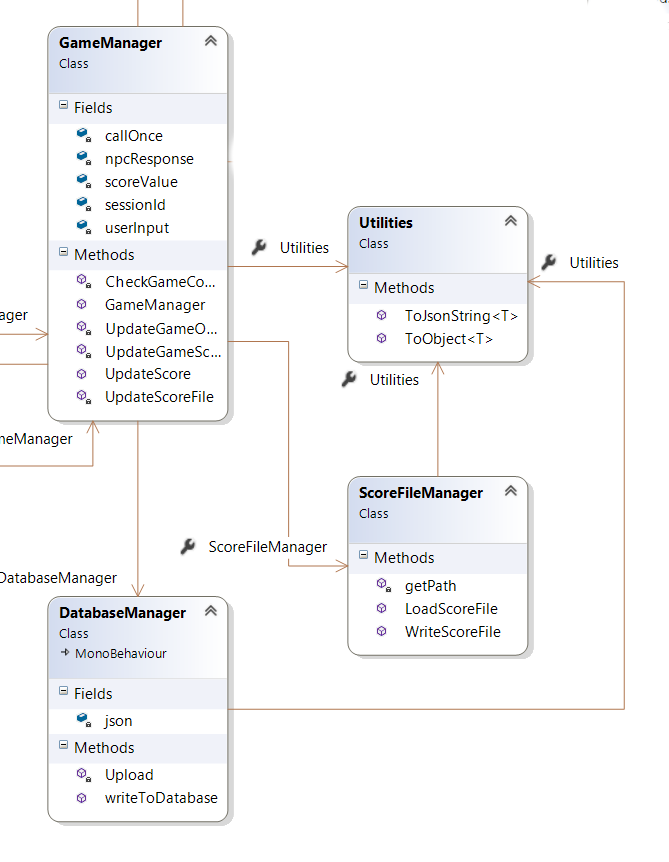
\includegraphics[width=0.8\textwidth]{Images/ClassDiagram Database.png}
\end{figure}

\section{Code Design}
With our experience from a number of modules throughout our Software Development course, we have implemented our best knowledge in the following areas to provide a well written and efficient piece of software.

\subsection{Design Patterns and Principles}
A design pattern is blueprint used to solve common problems in software development. They are used to improve code readability and efficiency. 

\subsubsection{Singleton}
The Singleton pattern has been implemented in a number of cases that require one instance of it. For example this pattern can be seen in the AudioController script and in listing~\ref{lst:Singleton}. This would ensure there was only one instance of the class created as there should only be one audio system. It also allowed it to work easily across multiple scenes such as the tutorial and start menu.

A Singleton is created by creating a private constructor so that no other classes can create an instance of that class. The second step is to create a static instance of the class which acts as the constructor. If the instance is null then create and instance once and store it, so further calls access this cached instance. This can be seen again in listing~\ref{lst:Singleton}

\begin{lstlisting}[caption={Singleton - implemented in the AudioController script.},label={lst:Singleton},language=python]
public static AudioController Instance { get; private set; }

private void Awake()
{
    if (Instance == null)
    {
        Instance = this;
    }
}
\end{lstlisting}

\subsubsection{Single Responsibility Principle (SRP)}
SRP ensures that every class has one single purpose. E.g so there isn't classes that are handling multiple tasks. At all levels throughout the design SRP is upheld as every class has specific purpose that delegates to other classes as required.

\subsubsection{Open Close Principle (OCP)}
OCP allows classes to be open for extension but closed for modification. So multiple clients, databases, speech engines etc could be added without breaking the overall implementation.

\subsubsection{Dependency Inversion Principle}
No higher-level modules or scripts depends on a low-level module. 

\subsubsection{Law of Demeter}
No single function knows the whole navigation structure of the system. All common functionality is subjugated into multiple methods and reused where possible.

\subsection{Object Pooling}
To save on system memory in regarding the 3D objects in the Unity engine we decided to just object pooling. What this entails is loading one model into memory and it is just duplicated preventing us from having to instantiate a new model every time. An example of this in the project is the City chunk model that spawns when you are on the train. One chunk is instantiate and every other chunk is a copy of that first one. Once the copy is out of view it is then deleted, therefore saving more system memory. Another example of this can be seen in start screen with the NPC models walking in the station. There is only three models and the rest of them are copies of the initial models. This was extreme important from a system design point of view. The reason being, we were developing this application for the Oculus Quest. The Quest is currently running an old enough version of Android, Android 7.1.1 to be exact. Because the Quest is running on an mobile operating system with mobile level specifications we needed to make sure it ran smoothly and Object pooling helped us achieve this.

\subsection{Modularity}
Even though at a glance the project seems pretty glued down, meaning it is a training simulation for ticket inspectors and that it. However, the system is designed in such a way that certain components can be swapped and changed to give the user a different training experience. For example the, to change the dialog of the NPCs all you have to do is simply change their AIML scripts. Now you have bots that are not just passengers on a train. To further the modularity, the entire scene can be changed in Unity with different models to give a different feel. Those are the two only things you would have to change in the entire project to create a training simulation for any other line of work.

\subsection{Error Handling}

\subsection{Security}

\section{Platforms}
As we were developing for Windows, Android and VR with a focus on VR we had to ensure everything we developed would work on all platforms. This was a big challenge but we developed in such a way that out features would port across easily. However some features did have to be designed slightly different such as the watch menu implementation described above.

\subsection{Oculus Quest}
\subsection{Android}
\subsection{Windows}
